\section{Auswertung} 

\subsection{Überprüfung der Bragg-Bedingung}

\begin{flushleft}
    Im ersten Teil der Versuchsreihe wird die Braggbedingung überprüft. 
    Dazu wird das Maximum aus dem Spektrum bestimmt.
    Das Maximum muss sich beim Doppelten Winkel $2\theta = 28\unit{\degree}$ befinden, da der Einfallwinkel $\theta = 14\unit{\degree}$ beträgt.
\end{flushleft}

\begin{figure}[H]  
    \centering
    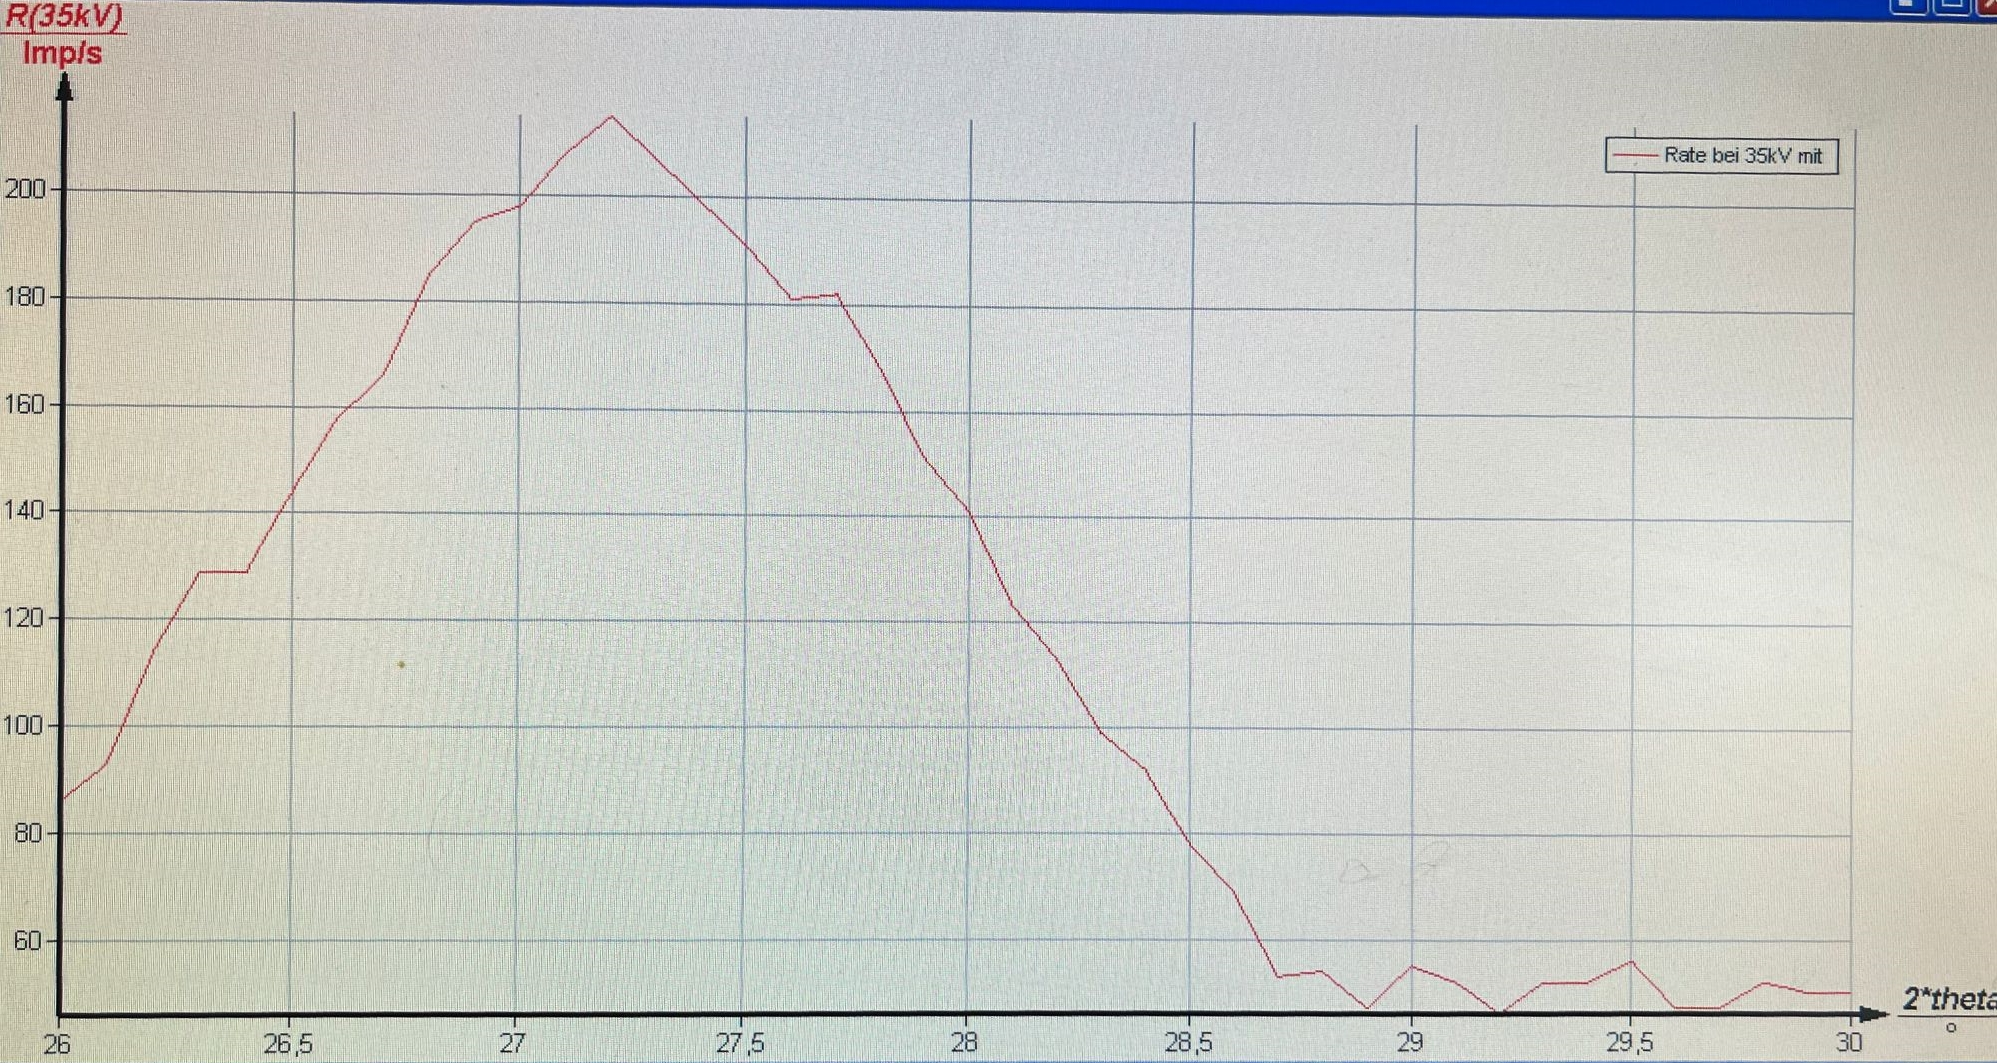
\includegraphics[height=70mm]{bilder/Bragg1.jpeg}
    \caption{Messkurve bei einem Einstellwinkel von  $\theta = 14\unit{\degree}$.\label{Abbildung2} }
\end{figure}

\begin{align*}
    \intertext{Aus der Abbildung \ref{Abbildung2} lässt sich der Winkel}
    \theta = (27,21 \pm 0,1)\unit{\degree}
    \intertext{ablesen.}
\end{align*}

\subsection{Emissionsspektrum einer Cu-Röhre}

\subsubsection{Maximalenergie des Bremsspektrums}

\begin{align*}
    \intertext{Um die Maximalenergie zu bestimmen wird der Winkel untersucht, bei dem sich die Intensität von null unterscheidet. 
    Dazu liegt das Emissionsspektrum in Abbildung \ref{Abbildung3} vor.
    Auffällig hierbei ist, dass es einenUnterschied bei dem Winkel}
    \theta_{1} = 8\unit{\degree}
    \intertext{gibt.
    Jedoch findet vorher eine minimale Änderungder Intensität bei dem Winkel }
    \theta_{2} = 6,6\unit{\degree}
    \intertext{statt.
    Daher werden beide Winkel als Relationswinkel gewählt.}
\end{align*}

\begin{figure}[H]  
    \centering
    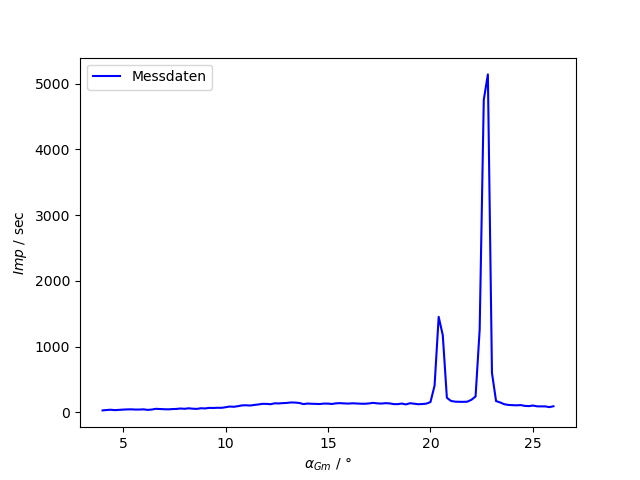
\includegraphics[height=80mm]{bilder/Emission.png}
    \caption{Emissionsspektrum der Cu-Röhre.\label{Abbildung3} }
\end{figure}

\begin{align*}
    \intertext{Aus der Formel (\ref{8}) folgt für die Energiewerte}
    \text{E}_{1} = 22,12\,\text{keV}\,, \\
    \text{E}_{2} = 26,79\,\text{keV}\,.
    \intertext{Dabei beträgt die minimale Wellenlänge, mit der Formel (\ref{1}) und $\text{e} \cdot \text{U} = 35\,\text{keV}$:}
    \lambda_{\text{min}} = 3,54 \cdot 10^{-11}\,\unit{\meter}\,.
\end{align*}

\subsubsection{Auflösungsvermögen des Apparatur}

\begin{flushleft}
    Zur Bestimmung des Auflösungsvermögen werden die Grenzwinkel, bei denen das Maximum auf die Härte ihres Wertes sunken, untersucht.
    Daraus ergibt sich für die Grenzwinkel mit den jeweiligen Energien nach (\ref{8}).
    Die Auflösungsenergie beschreibt das Verhältnis der Absorptionsenergie und der Energieänderung, die sich aus den Halbwertsbreiten bilden. 
    Die Auflösungsenergien sind in Tabelle (\ref{Tabelle}).
\end{flushleft}

\begin{table}[H] 
    \centering
    \caption{} 
    \label{Tabelle}
    \begin{tabular} {c  c  c  c  c  c  c}
        \toprule
        {$ $} &
        {$ \theta_{1} \mathbin{/} \unit{\degree} $} &
        {$ \theta_{2} \mathbin{/} \unit{\degree} $} &
        {$ \text{E}_{1} \mathbin{/} \text{keV}\ $} &
        {$ \text{E}_{2} \mathbin{/} \text{keV}\ $} &
        {$ A=\frac{\text{E}_{\text{k}}}{\increment \text{E}} $}&
        {$ \text{E}_{K} \mathbin{/} \text{keV}\ $}\\
        \midrule
        $\text{K}_{\beta}$  & 20,40 & 20,70 & 8,83 & 8,71 & 73,58 & 8,83 \\
        $\text{K}_{\alpha}$ & 22,41 & 22,93 & 8,07 & 7,90 & 46,76 & 7,95 \\
        \bottomrule
    \end{tabular} 
\end{table}

\subsubsection{Bestimmung der Abschirmkonstanten von Kupfer}

\begin{align*}
    \intertext{Aus der Abbildung \ref{Abbildung3} werden die Energien an der $\text{K}_{\alpha}$ sowie $\text{K}_{\beta}$ Linien bestimmt. 
    Durch das Ablesen der Winkel folgt für die Energien}
    \theta_{\alpha} = 22,8\unit{\degree}\,, \\
    \theta_{\beta} = 20,4\unit{\degree}\,,  \\
    \text{E}_{\text{K}_{\alpha}} = 7,95\,\text{keV}\,,  \\
    \text{E}_{\text{K}_{\beta}} = 8,83\,\text{keV}\,.  
    \intertext{Durch die Formel (\ref{5}) lassen sich die Abschirmkonstanten bestimmen. 
    Dabei ist $\text{Z} = 29$ die Ordnungszahl, $n=1$, $m=2$ und $l = 3$.
    Die Rydbergenergie beträgt $R_{\infty} = 13,6\,\text{eV}$.
    Die Abschirmkonstante $\text{E}_{\text{k, abs}}$ lässt sich nicht durch die Apparatur bestimmen, daher wird der Wert aus der Literatur \cite{a2} genommen mit $\text{E}_{\text{k, abs}} = 8,98\,\text{keV}$}
    \sigma_{1} = \text{Z} - \sqrt{\frac{\text{E}_{\text{k, abs}}}{\text{R}_{\infty}}} = 3,30\,, \\
    \sigma_{2} = \text{Z} - 2\sqrt{-\frac{\text{E}_{\text{K}_{\alpha}}}{\text{R}_{\infty}} + (\text{Z}-\sigma_{1})^2 } = 11,57\,, \\
    \sigma_{3} = \text{Z} - 3\sqrt{-\frac{\text{E}_{\text{K}_{\beta}}}{\text{R}_{\infty}} + (\text{Z}-\sigma_{2})^2 }  = 18,94\,.
\end{align*}

\subsection{Bestimmung der Abschirmkonstanten aus den Absorptionsspektren}

\begin{flushleft}
    Es werden für fünf Materialien (Zn, Ga, Br, Sr, Zr) jeweilige Absorptionsspektren erstellt und daraus die dazugehörige Abschirmkonstante mit Hilfe der Untersuchung der K-Kanten bestimmt.
    Die Bestimmung der Abschirmkonstanten erfolgt nach der Formel (\ref{5}) und der Energien nach (\ref{8}). 
    Die Winkel werden aus dem Spektrum ermittelt.
    Die ermittelten Werte werden tabellarisch in Tabelle \ref{Tabelle2} festgehalten.
    Die Absorptionsspektren sind wie folgt.
\end{flushleft}

\begin{figure}[H]
    \centering
    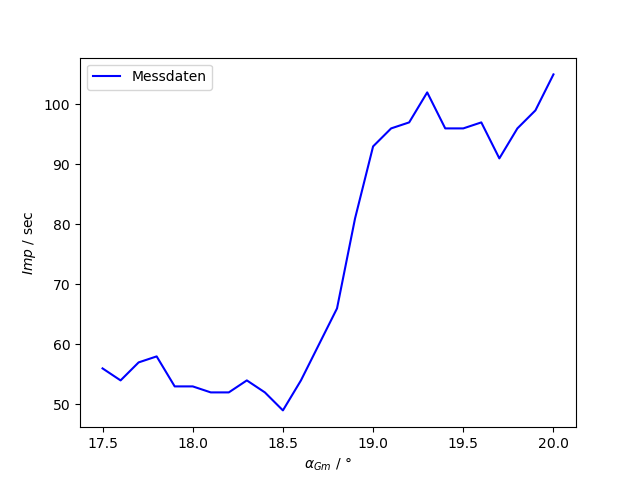
\includegraphics[height=80mm]{bilder/Zink.png}
    \caption{Absorptionsspektrum von Zink.\label{Abbildung4} }
\end{figure}

\begin{figure}[H]
    \centering
    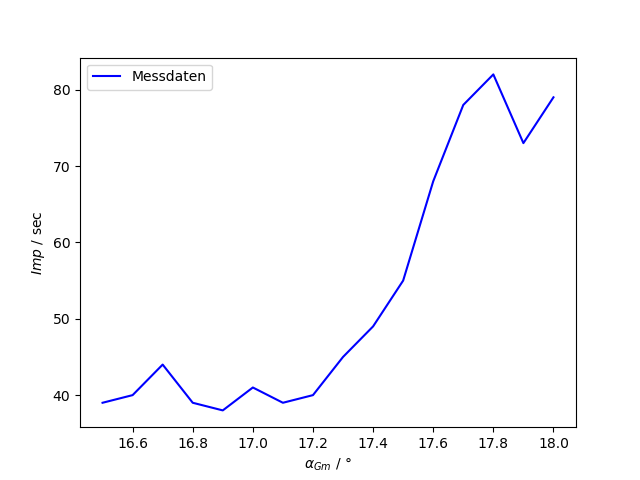
\includegraphics[height=80mm]{bilder/Gallium.png}
    \caption{Absorptionsspektrum von Gallium.\label{Abbildung5} }
\end{figure}

\begin{figure}[H]
    \centering
    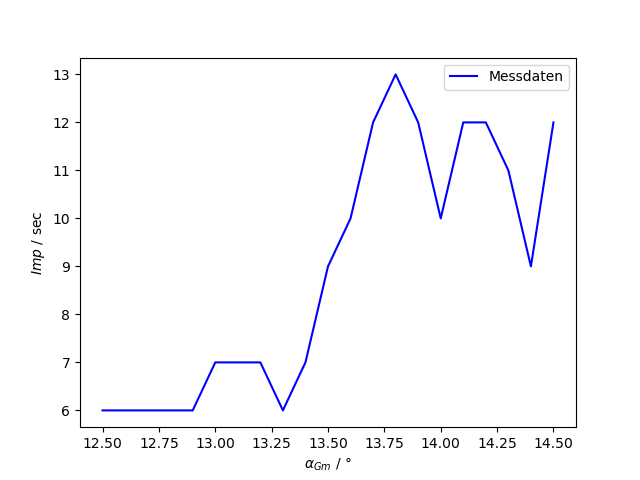
\includegraphics[height=80mm]{bilder/Brom.png}
    \caption{Absorptionsspektrum von Brom.\label{Abbildung6} }
\end{figure}

\begin{figure}[H]
    \centering
    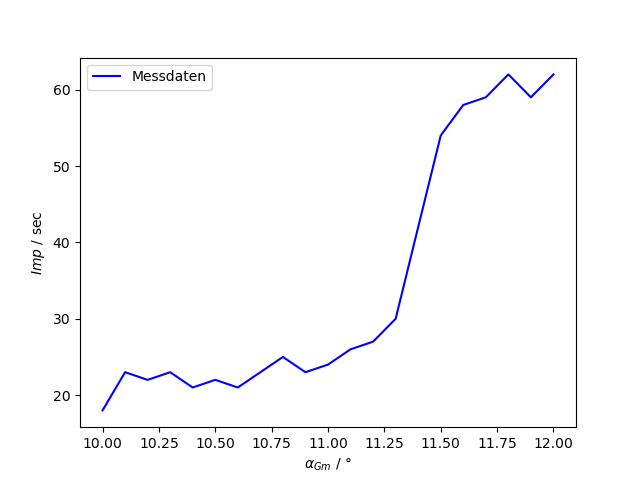
\includegraphics[height=80mm]{bilder/Strontium.png}
    \caption{Absorptionsspektrum von Strontium.\label{Abbildung7} }
\end{figure}

\begin{figure}[H]
    \centering
    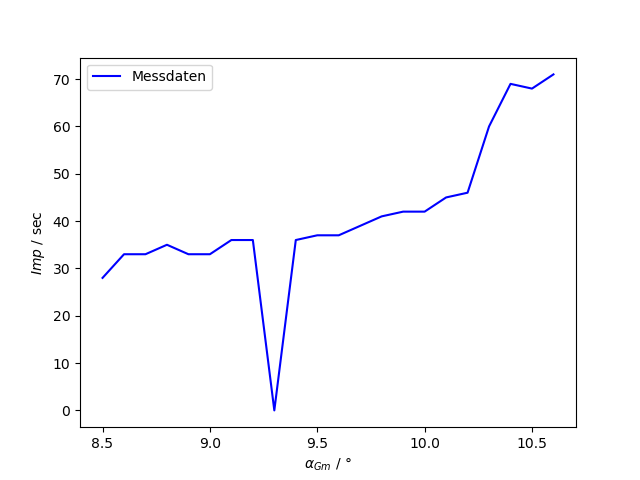
\includegraphics[height=80mm]{bilder/Zirkonium.png}
    \caption{Absorptionsspektrum von Zirkonium.\label{Abbildung8} }
\end{figure}

\begin{table}[H]     
    \centering
    \caption{Messwerte zu den jeweiligen Materialien.} 
    \label{Tabelle2}
    \begin{tabular} {c | c | c | c | c}
        \toprule
        {$  $} &
        {$ \text{Z} $} &
        {$ \theta \mathbin{/} \unit{\degree} $} &
        {$ \text{E} \mathbin{/} \text{keV}$} &
        {$ \sigma $} \\
        \midrule
        Zn & 30 & 18,82 & 9,54  & 3,51 \\
        Ga & 31 & 17,58 & 10,19 & 3,62 \\
        Br & 35 & 13,50 & 13,19 & 3,85 \\
        Sr & 38 & 11,44 & 15,52 & 4,21 \\
        Zr & 40 & 10,10 & 17,56 & 4,06 \\
        \bottomrule
    \end{tabular} 
\end{table}

\subsection{Bestimmung der Rydbergkonstante}

\begin{flushleft}
    Nach Moseley ist die Absorptionsenergie $\text{E}_{k}$ proportional zu $\text{Z}^2$.
    Die Energien werden in Abbildung \ref{Abbildung9} gegen die Ordnungszahlen aufgestellt.
\end{flushleft}

\begin{figure}[H]       
    \centering
    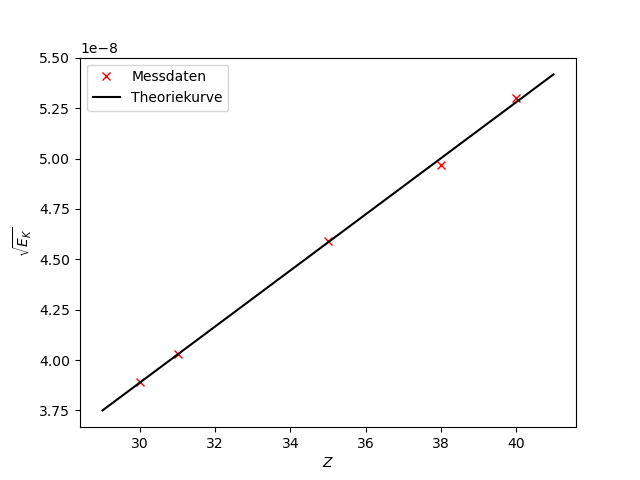
\includegraphics[height=80mm]{bilder/Rydberg.png}
    \caption{Energien in Wurzel gegen die Quantenzahl. \label{Abbildung9} }
\end{figure}

\begin{align*}
    \intertext{Die Steigung m der Gerade wird durch eine lineare Regression mit}
    \text{y} = \text{m} \cdot \text{x} + \text{n}
    \intertext{ermittelt}
    \text{m} = ( 1,38 \pm 0,02 ) \cdot 10^{-9} \sqrt{\text{J}}\,.
    \intertext{Die Rydberg-Konstante ergibt sich aus dem Moseleyschen-Gesetz}
    \text{R}_{\infty} = \frac{4\text{m}^2}{3\text{h}\nu},
    \intertext{somit}
    \text{R}_{\infty} = (1,27 \pm 0,48) \cdot 10^{7} \frac{1}{\text{m}}\,.
\end{align*}